% Study design and data flow: sources -> preparation -> analyses and checks -> outputs.
\documentclass[tikz,border=4pt]{standalone}
\usepackage[T1]{fontenc}
\usepackage{lmodern}
\renewcommand{\familydefault}{\sfdefault}
\usetikzlibrary{positioning,arrows.meta,fit,backgrounds}
\definecolor{violet}{HTML}{6D28D9}
\definecolor{cyan}{HTML}{0E8FAE}
\definecolor{ink}{HTML}{1B1E27}
\definecolor{grey}{HTML}{6B7180}
\tikzset{
  box/.style={draw=#1, fill=#1!8, rounded corners=3pt, line width=0.7pt, align=left,
    text width=4.1cm, inner sep=5pt, font=\footnotesize, text=ink, anchor=north},
  box/.default=grey,
  head/.style={font=\scriptsize\bfseries, text=grey, anchor=south},
  frame/.style={draw=grey!45, dashed, rounded corners=5pt, inner sep=6pt},
  arrow/.style={-{Stealth[length=2.8mm]}, line width=1pt, draw=grey},
}
\begin{document}
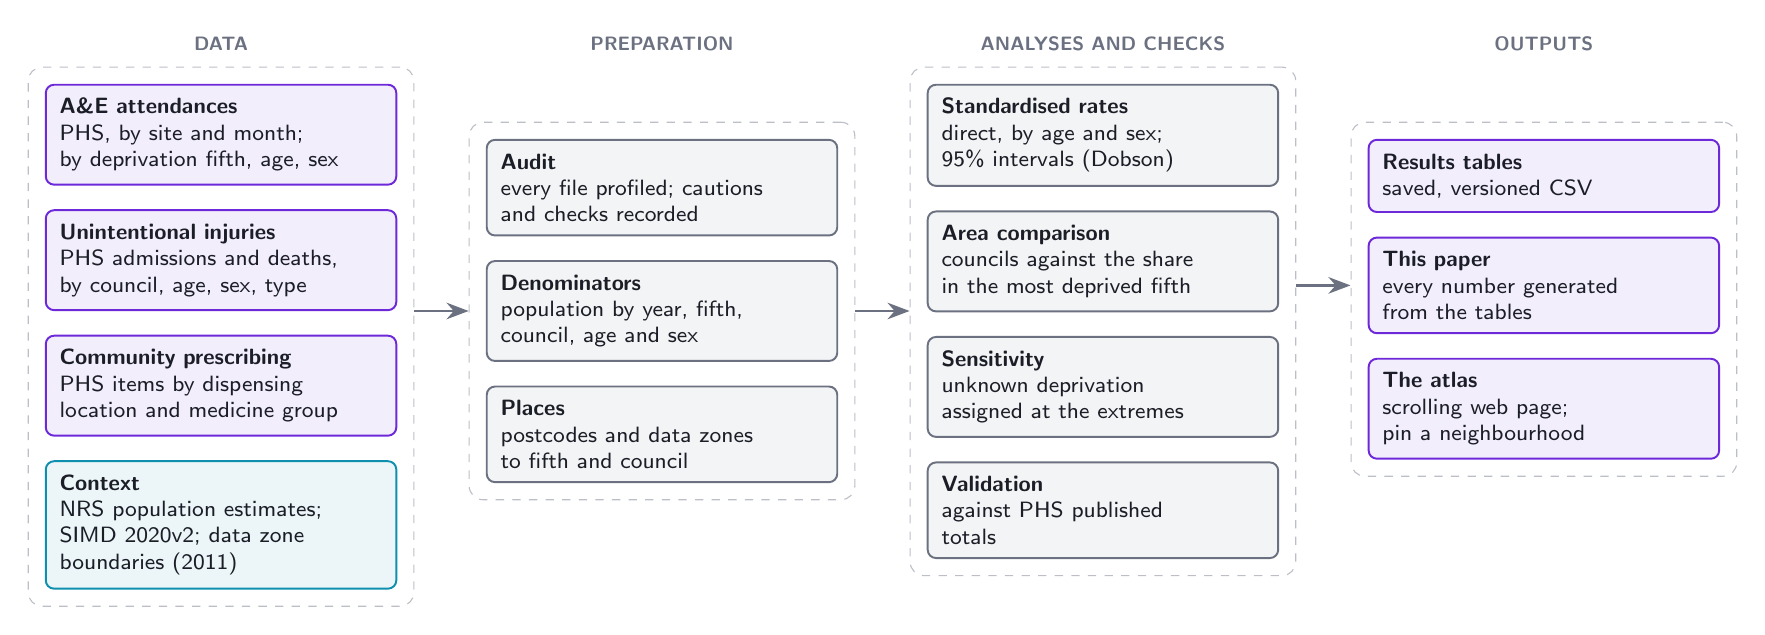
\begin{tikzpicture}[node distance=3mm]
  % column 1: data
  \node[head] (h1) at (0, 0) {DATA};
  \node[box=violet] (ae) at (0, -0.3) {\textbf{A\&E attendances}\\ PHS, by site and month;\\ by deprivation fifth, age, sex};
  \node[box=violet, below=of ae] (inj) {\textbf{Unintentional injuries}\\ PHS admissions and deaths,\\ by council, age, sex, type};
  \node[box=violet, below=of inj] (rx) {\textbf{Community prescribing}\\ PHS items by dispensing\\ location and medicine group};
  \node[box=cyan, below=of rx] (pop) {\textbf{Context}\\ NRS population estimates;\\ SIMD 2020v2; data zone\\ boundaries (2011)};

  % column 2: preparation
  \node[head] (h2) at (5.6, 0) {PREPARATION};
  \node[box] (audit) at (5.6, -1.0) {\textbf{Audit}\\ every file profiled; cautions\\ and checks recorded};
  \node[box, below=of audit] (den) {\textbf{Denominators}\\ population by year, fifth,\\ council, age and sex};
  \node[box, below=of den] (place) {\textbf{Places}\\ postcodes and data zones\\ to fifth and council};

  % column 3: analyses and checks
  \node[head] (h3) at (11.2, 0) {ANALYSES AND CHECKS};
  \node[box] (std) at (11.2, -0.3) {\textbf{Standardised rates}\\ direct, by age and sex;\\ 95\% intervals (Dobson)};
  \node[box, below=of std] (area) {\textbf{Area comparison}\\ councils against the share\\ in the most deprived fifth};
  \node[box, below=of area] (sens) {\textbf{Sensitivity}\\ unknown deprivation\\ assigned at the extremes};
  \node[box, below=of sens] (val) {\textbf{Validation}\\ against PHS published\\ totals};

  % column 4: outputs
  \node[head] (h4) at (16.8, 0) {OUTPUTS};
  \node[box=violet] (tables) at (16.8, -1.0) {\textbf{Results tables}\\ saved, versioned CSV};
  \node[box=violet, below=of tables] (paper) {\textbf{This paper}\\ every number generated\\ from the tables};
  \node[box=violet, below=of paper] (atlas) {\textbf{The atlas}\\ scrolling web page;\\ pin a neighbourhood};

  \begin{scope}[on background layer]
    \node[frame, fit=(ae)(pop)] (f1) {};
    \node[frame, fit=(audit)(place)] (f2) {};
    \node[frame, fit=(std)(val)] (f3) {};
    \node[frame, fit=(tables)(atlas)] (f4) {};
  \end{scope}

  \draw[arrow] (f1.east |- den.west) -- (f2.west |- den.west);
  \draw[arrow] (f2.east |- den.west) -- (f3.west |- den.west);
  \draw[arrow] (f3.east |- paper.west) -- (f4.west |- paper.west);
\end{tikzpicture}
\end{document}
